\documentclass{article}
\usepackage{amsmath}
\usepackage[utf8]{inputenc}
\usepackage{booktabs}
\usepackage{float}
\usepackage{microtype}
\usepackage{graphicx}
\usepackage{hyperref}
\usepackage[colorinlistoftodos]{todonotes}
\pagestyle{empty}

\title{Closest Pair Report}
\author{Adam Tovatt}

\begin{document}
  \maketitle

\section{Results}

All test cases passed when running the provided \texttt{check\_solution.sh} script. The program successfully solved even the largest test case with 1,000,000 points. On a modern machine, the total runtime for this case was around 1.4 seconds. The majority of the time is spent sorting the input points and computing the recursive closest pair distance. For example, for the largest input, the time spent on different parts of the solution is as follows:

\begin{tabular}{lrr}
\textbf{Section} & \textbf{Time (ms)} & \textbf{Percent of Total} \\
\hline
readInput           & 250   & 18.0\% \\
sortPoints          & 491   & 35.2\% \\
computeClosestDistance & 655   & 46.9\% \\
fullSolve           & 1401  & 100.2\% \\
\end{tabular}

\clearpage
\section{Implementation details}

I implemented a standard divide-and-conquer algorithm to solve the Closest Pair of Points problem. The input consists of up to 1,000,000 2D points, and the goal is to compute the smallest Euclidean distance between any two of them. The core steps are:

\begin{itemize}
  \item Sort the points by x-coordinate and y-coordinate at the beginning.
  \item Recursively divide the points into left and right halves.
  \item Compute the closest distance in each half.
  \item Construct a vertical strip around the midpoint and check potential cross-pair distances between the halves.
\end{itemize}

The main data structure used is a list of \texttt{Point} structs, and standard sorting algorithms are used to sort by x and y. The strip step only checks each point against at most 7 other nearby points thanks to geometric constraints.

The overall time complexity is \( O(N \log N) \), where \( N \) is the number of points. This comes from the recursive division (like mergesort) and a merge step that does linear work per level.

\subsection*{Discussion Questions}

\textbf{What is the time complexity, and why?} \\
The time complexity is \( O(N \log N) \). This is because the algorithm splits the data recursively (which takes \( \log N \) steps), and at each step it processes all \( N \) points by scanning the strip or combining results. Sorting the input initially also takes \( O(N \log N) \), and together this gives the final complexity.

\vspace{1em}
\textbf{Why is it sufficient to check a few points along the mid line?} \\
When checking for possible closest pairs that cross the dividing line, we only look at points within a narrow vertical strip of width \( 2\delta \), where \( \delta \) is the current best distance. Due to geometric packing limits in 2D, it's been proven that you only need to compare each point with at most 7 others in the strip (sorted by y-coordinate). Any additional points would be too far vertically to be closer than \( \delta \).

\vspace{1em}
\textbf{Draw a picture and show/describe when each distance is checked in your solution!} \\
In the recursive step, distances are checked between all pairs in the left half and in the right half. Then, in the "combine" step, distances are checked between points that lie near the dividing line (i.e., within \( \delta \) in the x-direction), and for those, only 7 ahead in the y-sorted list are checked. So each distance is checked either during brute-force (base case) or in the merge step when the point falls within the strip. \textit{(See the figures on the next page)}

\begin{figure}[H]
  \centering
  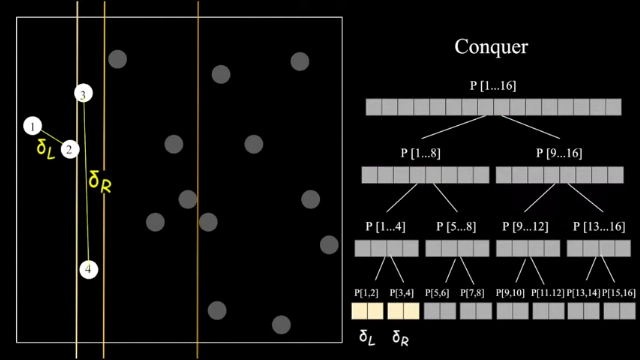
\includegraphics[width=0.9\textwidth]{figure1.png}
  \caption{Recursive case distance comparisson illustration. Taken from \href{https://www.youtube.com/watch?v=6u_hWxbOc7E}{this youtube-video} by Linq Qi also known as ``\href{https://www.youtube.com/@iDeer70}{``iDeer70''}.}
\end{figure}

\begin{figure}[H]
  \centering
  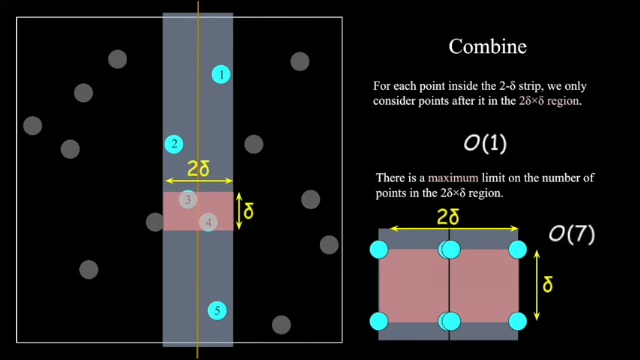
\includegraphics[width=0.9\textwidth]{figure2.png}
  \caption{Illustration of the strip search performed to ensure no closest pairs are missed due to the splitting. Taken from \href{https://www.youtube.com/watch?v=6u_hWxbOc7E}{this youtube-video} by Linq Qi also known as ``\href{https://www.youtube.com/@iDeer70}{``iDeer70''}.}
\end{figure}

\vspace{1em}
\textbf{When do you break the recursion and use brute force?} \\
The recursion breaks when the number of points in the subproblem is 3 or fewer. At that point, the function simply compares all pairs directly with brute force since the overhead of recursive division is not worth it for such small input.

\end{document}
